\section{Bernoulli Experiment and Binomial Distribution}

\subsection{The Bernoulli and Binomial Distributions}

If $p$ is the probability that an event occurs in a single trial (called the probability of success) and $q = 1 - p$ is the probability that this event does not occur in a single trial (called the probability of failure), then the probability that the event occurs exactly $x$ times in $N$ trials (that is, $x$ successes and $N - x$ failures occur) is given by
\begin{align}
 \label{eq:2.10.1}
 f(x)=P(X=x)=\comb{N}{x}p^{x}q^{N-x}
\end{align}
where $x=0,1,...,N.$

\begin{ejemplo}
  \label{exmp:2.10.1}
  The probability of obtaining exactly two heads in six tosses of a coin is
  \begin{align}
   \comb{6}{2}\left( \dfrac{1}{2} \right)^{2}\left( \dfrac{1}{2} \right)^{6-2}=\dfrac{15}{64}
  \end{align}
  using \eqref{eq:2.10.1} with $N=6, x=2, p=q=\frac{1}{2}.$
\end{ejemplo}

\begin{ejemplo}
 \label{exmp:2.10.2}
 Calculate the probability of obtaining at least 4 heads in 6 tosses of a coin.
\end{ejemplo}

\begin{solucion}
	Using the binomial distribution with $N=6$, $p=\frac{1}{2}$, $q=\frac{1}{2}$:
	\begin{align}
		P(X \geq 4) &= P(X=4) + P(X=5) + P(X=6) \\
		&= \comb{6}{4}\left(\frac{1}{2}\right)^4\left(\frac{1}{2}\right)^2 + \comb{6}{5}\left(\frac{1}{2}\right)^5\left(\frac{1}{2}\right)^1 + \comb{6}{6}\left(\frac{1}{2}\right)^6 \\
		&= \frac{15}{64} + \frac{6}{64} + \frac{1}{64} = \frac{22}{64} = \frac{11}{32} \approx 0.344
	\end{align}
\end{solucion}

In what follows, we will assume that we have imported the following packages:
\begin{itemize}
 \item \texttt{scipy.stats}
 \item \texttt{numpy} as \texttt{np}
\end{itemize}

\lstinputlisting[language=Python]{../code/distribuciones-especiales/statsBinom.py}

\begin{ejemplo}
  \label{exmp:2.10.3}
  Expand $\left( p+q \right)^{4}.$
\end{ejemplo}

\lstinputlisting[language=Python]{../code/distribuciones-especiales/coefBinom.py}

{Properties of the binomial distribution} Suppose we perform $N$ experiments with probability of success $p$ and probability of failure $q=1-p.$
\begin{align}
 \label{eq:2.10.2}
 \mu = Np \\
 \label{eq:2.10.3}
 \s^{2}=Npq
\end{align}

\lstinputlisting[language=Python]{../code/distribuciones-especiales/histBinom.py}

\begin{figure}
 \centering
 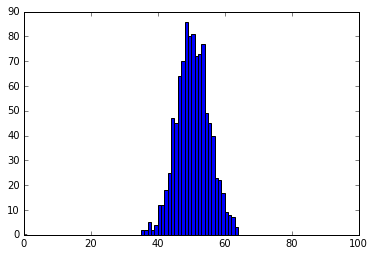
\includegraphics[height=7cm,keepaspectratio=true]{./pe/distBin01.png}
 % distBin01.png: 0x0 pixel, 300dpi, 0.00x0.00 cm, bb=
 \label{fig:2.10.1}
\end{figure}
